%----------------------------------------------------------------------------
\chapter{A JPorta (5-10 oldal)}\label{chapter:jporta}
%----------------------------------------------------------------------------

A BME Irányítástechnika és Informatika Tanszékén 2009 és 2015 között aktívan használták a CPorta névre keresztelt automatikus feladatkiértékelő rendszert, melyet a Közigazgatási Informatikai Központ (BME-IK) munkatársai fejlesztettek. Az idő folyamán a rendszert folyamatosan bővítették, azonban egy idő után ez egyre nehézkesebbé vált. Ennek oka a fejlesztőgárda cserélődése, a nem megfelelően átgondolt új funkciók implementálása, illetve az igények változása volt. Ezen okok miatt 2014-ben új portál fejlesztését kezdték meg a tanszéken \cite{KalmanMsc}.

 Így született meg a JPorta névre keresztelt oktatás támogató és automatikus feladat kiértékelő rendszer. A rendszer implementálása a Python programnyelv 3-as verziójával valósult meg, ezzel biztosítva a tartós támogatottságot. A webes felület generálásáért pedig a Django \cite{Django} keretrendszer 1.11.5-ös verzióját használja, amely ezen felül felelős a belső adatmodellen végzett műveletek adatbázisműveletekre fordításáért és végrehajtásáért is. 

 \section{Felépítés}

    \begin{figure}[h]
        \centering
        \resizebox{\textwidth}{!}{
            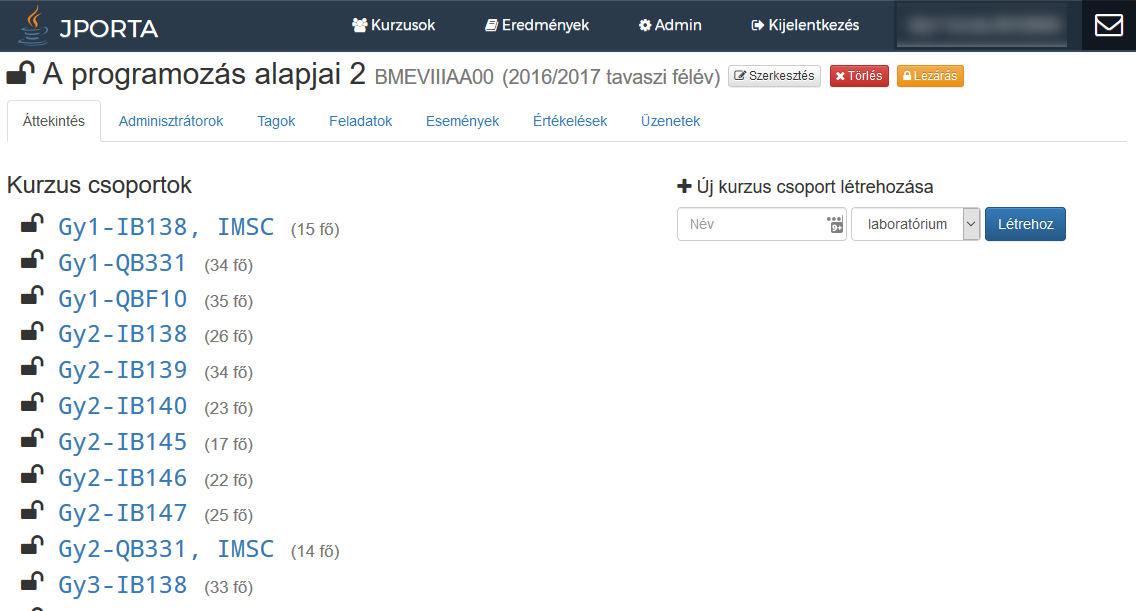
\includegraphics[]{jporta_course.png}
        }
        \caption{Tárgy adminisztrációs nézet}
        \label{fig:jporta_course}
    \end{figure}
     
    A portálon a felhasználókat négy csoportba sorolhatjuk: nem azonosított felhasználó, hallgató, oktató és adminisztrátor. A nem azonosított felhasználókat a portál azonosításra kényszeríti, mert számukra nincs elérhető tartalom. Az azonosításra jelenleg két mód áll rendelkezésre:
    \begin{itemize}
        \item BME címtár azonosítás \cite{BMECimtar}: ez az elsődleges azonosítási forma, ugyanis a célközönséget képző hallgatók és oktatók mind rendelkeznek ilyen fiókkal. Ennek köszönhetően egyszerűen, külön regisztráció nélkül hiteles adatokhoz juthatunk.
        \item Hagyományos felhasználói név és jelszó pár: ez a hitelesítési mód ritkán, csak kivételes esetekben használt. Ilyen lehet a portál bemutatására szánt próba felhasználói fiók.
    \end{itemize}

    A bejelentkezett felhasználók szerepelhetnek egyes tárgyaknál oktatói, másoknál hallgatói szerepben. Erre sok esetben szükség is van, hiszen a laboratóriumi foglalkozásokat és gyakorlatokat gyakran felsőbb éves hallgatók tartják.

    A JPorta keretein belül a Neptun rendszerhez hasonló tárgy-kurzus struktúra került implementálásra, azaz létrehozhatóak tárgyak, majd ezeken belüli további kurzusok a gyakorlatok, laboratóriumi foglalkozások számára (ld. \ref{fig:jporta_course}. ábra). A tárgyakhoz és a kurzusokhoz külön-külön rendelhetünk oktatókat. Előbbi esetben a teljes tárgyat kezeli az adott személy, utóbbi esetben csak a kurzusában lévő hallgatókat.
    
    A kurzusokhoz hozzárendelhetünk különböző számonkérések és jelenlétek eredményét, ezekből készített dinamikusan számolódó mezőket, illetve automatikusan kiértékelődő feladatokat. Ezekről részletesebben \aref{chapter:assessments}. és \aref{chapter:exercise}. fejezetben lesz szó.
     
\section{A rendszer hallgatói oldalról}
    A portálra belépve a hallgatókat egy összefoglaló nézet fogadja (ld. \aref{fig:jporta_home}. ábra). Itt lehetőségük van az aktív és korábbi online beadandó feladataikat megtekinteni. Itt láthatják a részletes eredményüket is, illetve (ha a határidő még nem járt le) leadhatnak új megoldást is.
    
    \begin{figure}[h]
        \centering
        \resizebox{\textwidth}{!}{
            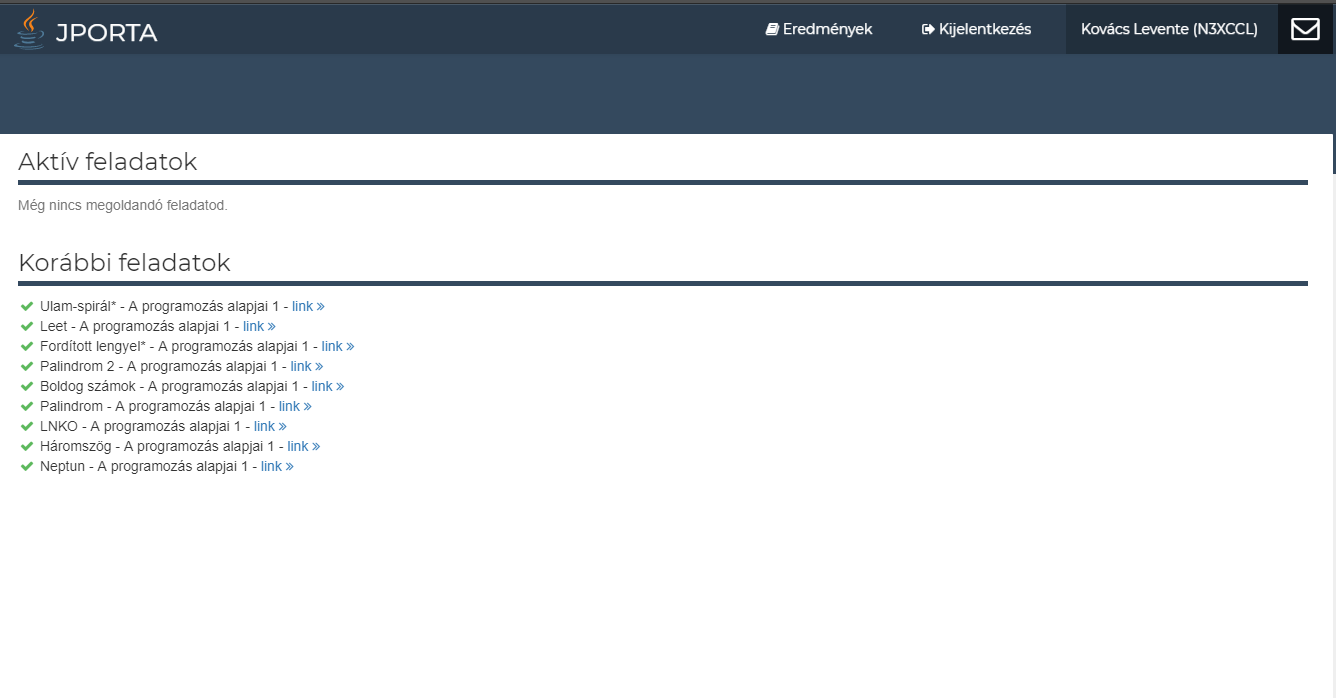
\includegraphics[]{jporta_home.png}
        }
        \caption{Belépő képernyő}
        \label{fig:jporta_home}
    \end{figure}
 
\section{A rendszer oktatói oldalról}
    Az oktatóknak lehetősége van a tárgyukhoz, vagy kurzusukhoz tartozó hallgatók értékelésére. Ebbe beletartozik a különböző zárthelyi dolgozatok eredményének beírása, a jelenlétek vezetése, illetve az automatikusan kiértékelődő feladatok ellenőrzése, esetleges felülbírálása.